\chapter{Introduction}
\label{cha:introduction}


\section{Background}

As companies and consumers increasingly purchase goods online, the demand for cross carrier management platform
delivery services grows (First Research 2013, 7). Furthermore, the growth of online retail
sales has influenced the logistics industry for the past ten years and the trend is expected to
continue at least on a similar level during the next few years. (Delfmann et al. 2002, 203.) 

\begin{figure}[!ht]
	\centering
	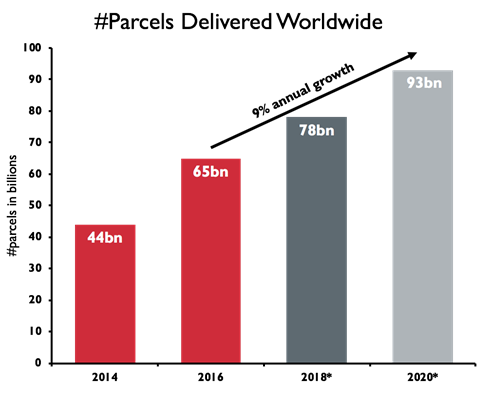
\includegraphics[width=0.5\textwidth]{images/ParcelsDel.png}\\
	\caption{Parcels Delivered worldwide [billions]}
	\label{fig:introduction__loremipsum}
\end{figure}

Responding to the increased demand of small-sized frequent shipments incurred by e-commerce has become one of the biggest challenges for logistics express delivery companies.
A successful delivery of shipments to consumers distributed across large geographical areas
will require re-designing of the existing system.

The increase of business-to-consumer (B2C) e-commerce activities implies that business are border less, global ecommerce is selling products or offer services across the world, in many case without anyu


The idea to investigate delivery service based on the  blockchian proposed by the the Tu Berlin. The DC3 team in this project did not focused in implementing the blockchian system but rather in creating a platform interface to manage the parcel. as today each company store the parcel data in her own local servers, only basic parcel data    






\section{Problem Discussion}

\subsection{Vendors communication and limitations}
There are multiple inefficiencies in cross-border delivery industry, related to lack of transparency and trust between the different logistics providers. International parcel delivery usually go through several logistics vendor, each on their side of the border, and there is a lot of accounting and interoperability overhead in the interactions between the different vendors. The idea is to solve these issues with the blockchain technology, taking advantage of its inherent transparency and trust.
From a Logistic company perspective, the parcel information is limited to their ownership and post completion of handover to a peer logistic company the package would not be efficiently tracked and the interrelated companies handling the package would not be in consensus. This common interface provides a plausible solution to the problem stated above by giving an opportunity for the companies to keep track of the package irrespective of the ownership of the package at a given point of time by having full information about it. It will also help the companies achieve better customer satisfaction by providing such sensor options to its customers to make use of.

\subsection{Vendors HMI}
From a customer perspective, when a customer orders a parcel the information revealed to him is depended on the quality of the carrier web interface, with a unique high-detailed dashboard the customer can be independent from the retail interface system and be informed about the status of the package and location of the package at all times throughout the journey of the package from source to destination.More options are made available to the customer in terms of a temperature and a shock sensor which is capable of taking lower and upper limits from the customer as an input and reverting with any irregularities in the package.

% \begin{table}[!ht]
% 	\small
% 	\centering
% 	\begin{tabular}{|l|l|l|l|}
% 		\hline
% 		Lorem & ipsum & dolor & sit \\
% 		\hline
% 		amet & consetetur & sadipscing & elitr \\
% 		\hline
% 		Lorem & ipsum & dolor & sit \\
% 		\hline
% 		amet & consetetur & sadipscing & elitr \\
% 		\hline
% 	\end{tabular}
% 	\caption{Lorem ipsum...}
% \end{table}


% \subsubsection{Even more Lorem Ipsii}

% alon
